%! TEX program = xelatex

\documentclass[../Postbot.tex]{subfiles}

\begin{document}

    \begin{frame}
        \frametitle{场景介绍}
        \begin{columns}
            \begin{column}{.4\linewidth}
                国内社交媒体 \\
                \hspace*{\fill} \\
                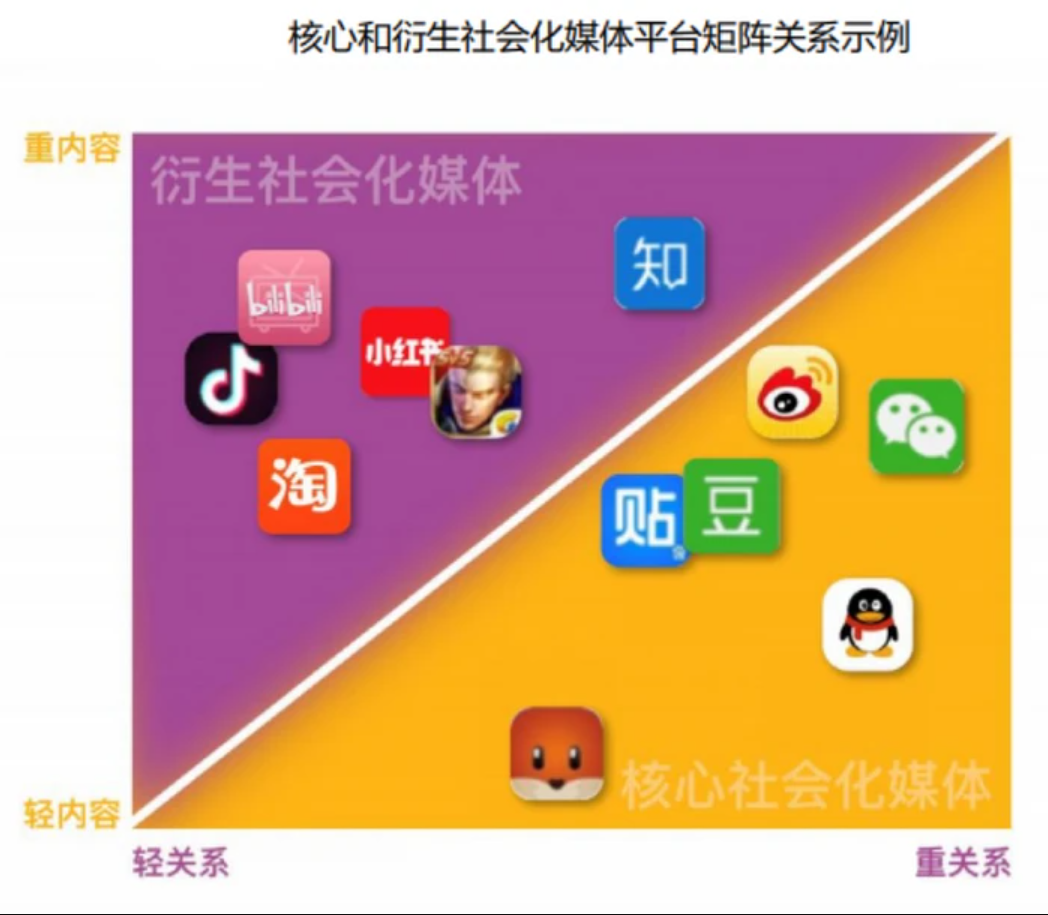
\includegraphics[scale=0.2]{../src/img/Social_media_mainland.png}

            \end{column}
            \begin{column}{.4\linewidth}
                海外社交媒体 \\
                \hspace*{\fill} \\
                \hspace*{\fill} \\
                
\includegraphics[scale=0.07]{../src/img/Social_media_oversea.jpg}

            \end{column}
        \end{columns}
    \end{frame}

    \begin{frame}
        \frametitle{场景介绍}
        \begin{columns}
            \begin{column}{.3\linewidth}
                {\large 一个“帖子”的可能元素} \\
                \hspace*{\fill} \\
                \begin{itemize}
                    \item 文字
                    \item 图片
                    \item 短视频
                    \item tag
                    \item 超链接
                    \item ……
                \end{itemize}

            \end{column}

            \begin{column}{.5\linewidth}
                
                \begin{figure}[h]
                    \centering
                    
\includegraphics[scale=0.24]{../src/img/Facebook.png} \\
                \end{figure}

                \begin{figure}[h]
                    \centering
                    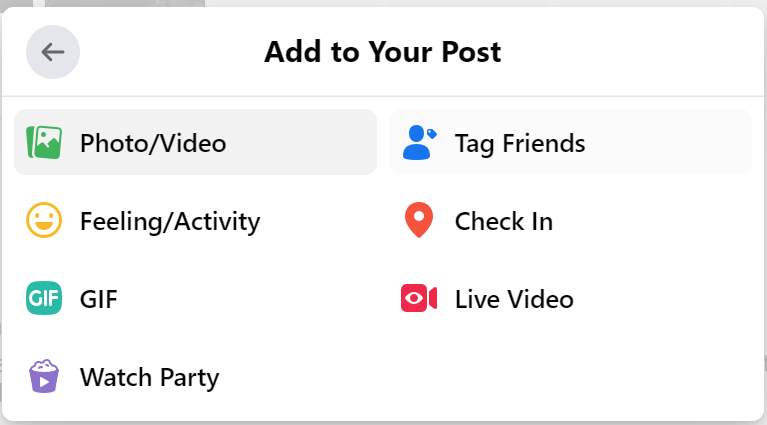
\includegraphics[scale=0.24]{../src/img/Facebook_extension.png} \\
                \end{figure}

                \begin{figure}[h]
                    \centering
                    
\includegraphics[scale=0.24]{../src/img/Tweet.png}
                \end{figure}
            \end{column}
        \end{columns}
    \end{frame}

\end{document}